\documentclass[11pt,a4paper]{report}

% Aberstwyth MMP Project Report Template for LaTeX
%
% Authors: Neil Taylor (nst@aber.ac.uk) and Dr. Hannah Dee (hmd1@aber.ac.uk) 
%
% This has been adapted from the Leeds Thesis template and the 
% Group Project template for Computer Science in Aberystywth University.
% 
% All comments and suggestions welcome.
%
% Template designed to be used with pdflatex: it may need alteration to
% run with a different LaTeX engine.
%
% Note - this is offered as a starting point for your work. You are not 
% required to use this template and can choose to create your own document 
% without it.

% This template is suitable for students with an engineering-style project, 
% which will be most students in the department. If your project is a research-oriented 
% project, look at the alternative template.

% To build document on the unix command line, run four commands:
 
% pdflatex mmp-report
% bibtex mmp-report
% pdflatex mmp-report
% pdflatex mmp-report

% you will end up with mmp-report.pdf. Before submitting, add your user ID as a prefix, 
% e.g. abc01-mmp-report.pdf 
\usepackage{StylesAndReferences/mmp-report}

% the following packages are used for citations - You only need to include one. 
%
% Use the cite package if you are using the numeric style (e.g. IEEEannot). 
% Use the natbib package if you are using the author-date style (e.g. authordate2annot). 
% Only use one of these and comment out or remove the other one. 
\usepackage{cite}
%\usepackage{natbib}

%%%% Title and Section Colours %%%%
% Modify these values to change the colours used for title, sections and subsections.
% Each value is a range of 0-255 in RGB colourspace.
% Idea courtesy of discussion at 
% https://www.overleaf.com/learn/latex/Using_colours_in_LaTeX
% and
% https://tex.stackexchange.com/questions/75667/change-colour-on-chapter-section-headings-lyx
% 
% If you prefer to have black headers, then comment out the following lines
\definecolor{mmpTitle}{RGB}{10, 85, 145}
\definecolor{mmpSection}{RGB}{10,85,155}
\definecolor{mmpSubsection}{RGB}{79,129,189}

\chapterfont{\color{mmpTitle}}  % sets colour of chapters
\sectionfont{\color{mmpSection}}  % sets colour of sections 
\subsectionfont{\color{mmpSubsection}} % sets colour subsections
\subsubsectionfont{\color{mmpSubsection}} % sets colour subsections

%%%% end of Title and Section Colours %%%%


%%%% Report Type %%%%
%% comment/uncomment depending on the type of report you want to generate
\reporttype{Engineering}
%\reporttype{Research}
%%%% end of Report Type %%%%


\begin{document}

%TC:ignore

% all of the include directives below refer to tex files
% so %TC:ignore 

\title{ESP32 Lighting Controller}

% Your name
\author{Kieran Todd}

% Your email 
\authoremail{ktt1@aber.ac.uk}

\degreeschemecode{G400} %e.g. G400 
\degreeschemetitle{Computer Science} % e.g. Computer Science
\degreetype{BSc}

\modulecode{CS39440} % i.e. CS39440, CC39440, CS39620
\moduletitle{Major Project} % i.e. Major Project or Minor Project

\date{20th April 2021 } % i.e. the date of the current version of your report

\status{Release} % Use draft until you create the release version. Then, change this to Release.
\version{4.0}

% The title and name of your supervisor.
\supervisor{ Richard Shipman} 

%The email for your supervisor. 
\supervisoremail{rcs@aber.ac.uk}

\maketitle

%TC:endignore
 includes cover.tex - to change the content,
% edit the tex file

\pagenumbering{roman}

% This is the front page
%TC:ignore 

\title{ESP32 Lighting Controller}

% Your name
\author{Kieran Todd}

% Your email 
\authoremail{ktt1@aber.ac.uk}

\degreeschemecode{G400} %e.g. G400 
\degreeschemetitle{Computer Science} % e.g. Computer Science
\degreetype{BSc}

\modulecode{CS39440} % i.e. CS39440, CC39440, CS39620
\moduletitle{Major Project} % i.e. Major Project or Minor Project

\date{20th April 2021 } % i.e. the date of the current version of your report

\status{Release} % Use draft until you create the release version. Then, change this to Release.
\version{4.0}

% The title and name of your supervisor.
\supervisor{ Richard Shipman} 

%The email for your supervisor. 
\supervisoremail{rcs@aber.ac.uk}

\maketitle

%TC:endignore
                        

% Set up page numbering
\pagestyle{empty}

% declarations of originality 
\thispagestyle{empty}

%TC:ignore

%%%
%%% You must sign the declaration of originality. 
%%%
%%% You are submitting this electronically. Therefore, to sign, you 
%%% type your name and date to replace the .... characters. 
%%%
\section*{\centering Declaration of originality}

I confirm that:

\begin{itemize}
\item{This submission is my own work, except where 
clearly indicated.}

\item{I understand that there are severe penalties for Unacceptable Academic Practice, which can lead to loss of marks or even the withholding of a degree.}
 
\item{I have read the regulations on Unacceptable Academic Practice from the University's Academic Registry (AR) and the relevant sections of the current Student Handbook of the Department of Computer Science.}
 
\item{In submitting this work I understand and agree to abide by the University's regulations governing these issues.}
\end{itemize}

\vspace{2em}
Name: Kieran Todd \\

\vspace{1em}
Date: 30th April 2021 \\

%%% 
%%% We would like to make a selection of final reports available to students that take 
%%% this module in future years. To enable us to do this, we require your consent. You 
%%% are not required that you do this, but if you do give your consent, then we will have 
%%% the option to select yours as one of a number of reports as examples for other 
%%% students. If you would like to give your consent, then please include the following 
%%% text and type your name and date to replace the .... characters. 
%%% 
%%% If you do not wish to give your consent, please remove this from your report. 
%%%
\vspace{1em}
\section*{\centering Consent to share this work}

By including my name below, I hereby agree to this project's report and technical work being made available to other students and academic staff of the Aberystwyth Computer Science Department.  

\vspace{2em}
Name: Kieran Todd \\

\vspace{1em}
Date: 30th April 2021\\

%TC:endignore

               

\thispagestyle{empty}

%TC:ignore

\section*{\centering Acknowledgements}

I am grateful to all of the computer science lectures that have helped during my time at Aberystwyth. Specifically I would like to thank Neil Taylor and Richard Shipman. Neil Taylor has helped me and understood me whenever I have had hard times throughout the year and has truly been a supportive head of year. Richard has been a fantastic supervisor during this project, and I am thankful for his support and advice.

I would also like to thank one of my closest friends at university, Ryan Priest, for keeping me sane (mostly) over the last 4 years.

Lastly I am grateful towards my mother who has always supported me thought my time at university and has helped me in whatever way she can.


%TC:endignore % Acknowledgements

\thispagestyle{empty}

%TC:ignore

\section*{\centering Abstract}

This report aims to outline the process and the decisions made through the duration of my ESP32 lighting controller that was created in the Arduino IDE environment. The aim of the project was to make a fully customisable light emitting diode (LED) controller, with two different LED output options, for the use in dioramas and model scenarios. These LED sequences could either be played constantly, or a trigger could be set on the LED profile. These triggers have  parameters that define under what conditions the LEDs would display its LED sequence. The program also has a website front end, that was hosted from the ESP32, that allows the user to create and edit the LED profiles and define the triggers and its parameters.

The program has the ability for expansion to include other types of triggers and outputs. In the planning section of the project, ideas were included to implement servos, motors and sound into a range of the output options. The ideas suggested allowed for moving parts to be displayed via a trigger in a similar way as the LED profiles were activated. Also with the addition of sound, a MP3 file could be triggered when a profile was displayed. On completion, this would allow for the user to create displays like a level crossings with rising barriers, flashing lights and a warning sound preformed when a train passes by. These features did not get implemented however, as they did not fit within the timescale of the project. 


%TC:endignore                 % Abstract

\pagenumbering{roman}
\pagestyle{fancy}
\fancyhead{}
\fancyfoot[C]{\thepage}
\renewcommand{\headrulewidth}{0 pt}
\renewcommand{\chaptermark}[1]{\markboth{#1}{}}

\tableofcontents   
\newpage
\listoffigures % comment out this line if you don't have any figures / graphics
\newpage 
\listoftables % comment out this line if you don't have any tables
\newpage

% Set up page numbering
\pagenumbering{arabic}

\setchapterheaderfooter

%TC:endignore

% include the chapters
\chapter{Background \& Objectives}
\section{Background}
The aim of the project was to make a fully customisable light emitting diode (LED) controller for the use in dioramas and model scenarios. It was essential to build capacity within the program that allowed for future expansion to accommodate a range of outputs and inputs. The concept of the program was to enable the user to create many lighting sequences. The lighting sequences consisted of a range of brightness levels and an assortment of colours. A feature of the program was to ensure there were minimal constraints on the creation on the lighting sequences as possible. The user set this lighting sequence to display on a specific LED. Also, the user was able to define the conditions under which the LED profile would play (the LEDs trigger). Some of the base triggers initially formulated were time, temperature, weather, button and constant.

The concept behind the customisable LED controller came from the current marketplace for model LED setups. Malcom Miniatures are the manufacturers of one of the most popular LED controllers on the marketplace \cite{MMinitures}. However, these controllers are limited as they display only two lighting sequences i.e. candles and fire. The lighting sequences can only be displayed on standard LEDs. The controller has no functionality or expandability to allow for the use of assignable LEDs. Also, these LEDs were restricted to either being ‘on’ or ‘off’; there was no way of assigning a condition to the program that allowed the user to control how the lighting sequence was displayed. This was undesirable as having LEDs powered constantly could be seen as an eyesore, unimaginative or not engaging for the user. Also, turning the unit on and off could have been a burden.

\section{Analysis}
The program was created on the ESP32 microcontroller. The reason it was used over the other brands of microcontrollers was due to the following reasons:

\begin{itemize}
\item In-built WIFI capability - The ESP32 has WIFI funtionality attached to the microcontoller. This is benificial as the program was able to host a website front end without the use of an external WIFI card. 

\item Numerous output pins with pulse width modulation (PWM) enabled - On the ESP32 there were more PWM pins than most other microcontrollers. This allowed the use of a greater number of standard LEDs. The LEDs were assigned a sequence of brightness that were displayed rather than being fixed at an ‘on’ or ‘off’ state. 

\item End-user specification - In the initial project specification the microcontroller that was identified as a 'must have' was the ESP32. This was due to the reasons outlined above. 
\end {itemize}

The main reason the ESP32 microcontroller was selected over the other brand of micro controllers (other than the in-built WIFI capacity) was because, as stated above, the ESP32 has more PWM pins. Comparatively, if we look at other micro controllers like the ESP8266(4 PWM pins) and the Arduino Nano(6 PWM pins) have a fraction of the PWM pins comparted to the ESP32 (25 PWM pins). 

The program created allowed for two different LED outputs: standard LEDs and addressable LEDs. The operation of the LEDS by a user was via a website. Standard LEDs are regular LEDs with a fixed colour. When powered, these LEDs display a brightness which is fixed to either a High (on) or Low (off) state. Addressable LEDs display a colour. The use of three different variables, red, green or blue, defines the colour output on the addressable LEDs. For example, if a purple output was required then the red and blue values were set to a high value while the green value was set to zero. 

The standard LEDs and addressable LEDs were connected to the ESP32 microcontroller output pins. Some of the output pins on the ESP32 have pulse width modulation (PWM) enabled, which allowed us to display a brightness from 0 (off) to 255 (brightest setting) on the standard LEDs. PWM allowed us to reduce the power delivered to the standard LED by having it powered ‘off’ and ‘on’ multiple times a second. The longer the time the LED was ‘off’ compared to ‘on’ gave a dimmer LED. However, when the LED was powered ‘on’ for a longer amount of time than ‘off’, this displayed a brighter LED.

Both standard and addressable LED profiles have a brightness/colour sequence of an undefined length. Each LED profile displayed the next colour/brightness in the array after a specified amount of iterations had passed. An iteration is one of the repetitions of a process that generates a specific outcome. In this program an iteration was one of the many times the program went through the main lighting loop. When creating the LED profile, the user defined how many iterations through the main lighting loop it would take before moving on to the next colour/brightness e.g. each iteration of the main LED array was set to take 200 milliseconds and the next brightness/colour was displayed after three iterations, therefore each brightness was displayed for 600 milliseconds (0.6 seconds) before moving on to the next colour/brightness in the array. 

The program allowed for the use of servos to move parts within a diorama e.g. a level-crossing barrier or a character. If the user were defining a servo profile, the user would set the degree (angle) the servo would turn to and the speed at which it would move. Also, the program allowed for the use of motors. The motors allowed for scenes such as lighthouse lights or a merry-go-round to revolve around a point at a defined speed for a specified length of time. Both the servo and the motor had a trigger, just like the LED profiles, to which it performed the desired reaction when the trigger was true.

Each LED was assigned a LED profile by the user which performed a specific action when a specified trigger came into fruition. Each of these profiles were given a ‘trigger’ which defined what conditions the LED started displaying its lighting/ brightness sequence. The standard triggers were:
\begin{itemize}
\item Time- The user defines a start and an end time. When the geographical time falls between the start and end time, the LED profile plays continuously. Once the geographical time surpasses the end time, the LED switches off.
\item Weather - The user selects a location and is given a list of different weather states. When the weather in the defines location matched the correct state the LED profile played until the weather changes.
\item Temperature - The user defines a temperature in degrees Celsius. They also define whether they would like the profile to trigger when the current temperature is above or below the defined trigger. 
\item Button – The button used by the program has two states. When activating the button (in its ‘on’ state) the profile plays. When deactivating the button (in its ‘off’ state) the profile ceases to play. 
\item Constant – The LED plays continuously when the trigger is set to constant.
\end {itemize}

The aim of the website was to give the user a manageable way of changing the triggers and LED brightness/colour levels as stated above. The user was able to change, retrieve and edit the LED profiles and then assign LED profiles to the respective LEDs easily. The main purpose of the website was for any user to be able to understand and navigate the website controls even if they have a limited computer knowledge.

\section{Process}
The process that was adopted to complete the project was the agile methodology. Other methodologies considered were incremental development and continuous integration. The agile methodology was preferred as its main features include rapid production of working code and emphasis on what the customer would want. Specifically, it was decided that Scrum agile methodology would be used. However, this methodology had to be adapted slightly as Scrum was created for use in small teams not a singular person. After reading a helpful and easy to read article on "Scrum for One" by Alex Andrews \cite{Scrum}, it was decided to adopt Scrum with the following changes:

\begin{itemize}
\item Daily scrum - This is a personal five-minute review of what was completed yesterday, specifically the elements that did not get completed, then plan the task(s) for the day prioritising what was not completed previously.
\item Sprint - This is completed in the same way as a normal scrum; it is just trying your best to accomplish what was proposed during the daily scrum.
\item Story time - Normally completed at the end of the week, Story time was time spent away from the desk thinking about the implementation of features and tasks for the next sprint week.
\item Release - This time was spent with the customer (my supervisor) explaining the tasks completed, future tasks and problems encountered.
\item Sprint plan- This was where the plan for the next week’s sprint tasks were completed.
\end {itemize}

\chapter {Requirements}
At the beginning of this project, a list of requirements was defined. It was then decided that a MoSCoW analysis would be performed on the list of requirements. Each requirement was given one of the four letters which are:
\begin{itemize}
\item M - Must have - This is the highest priority letter. These requirements were necessary to the completion of the project and must be prioritised.

\item S - Should have - These requirements were not vital to the completion of the project but were features and additions that were expected to be completed by the end of the project.

\item C - Could have - The 'could have' requirements were desirables that were not vital to the completion of the project but were additions to the project that made it function better. 

\item W - Will not have - The lowest priority letter. these requirements were normally out of the scope of the project and were too ambitious for the time frame so they would not get completed.
\end{itemize}
This analysis helped me understand what requirements should be focused on and gave a better picture of what the final product may look like. Requirement one to seven are requirements of the code, while requirement eight to sixteen are website requirements.

\section {RQ1 - ESP 32 must react to the changes made by the user (M)}
When a LED configuration is changed an any way (trigger/trigger parameters changed, profile changed, LED attached) the ESP32 responds to these changes and displays the new LED configuration correctly. 

\section {RQ2 - Display the brightness and the colours of the LEDs correctly (M)}
When the brightness or the colour of the LEDs change, for example when the display moves on to the next section of the array, the LEDs will display the new brightness/colour in the intended way.

\section {RQ3 - Perform defined output when trigger is met. (M)}
While a trigger is active, the LED brightness/colour sequence is displayed to the LED.

\subsection {RQ3.1 - Time trigger(S)}
The user defines a start time and an end time, when the geographical time falls between these two times the trigger is considered active. 

\subsection {RQ3.2 - Weather trigger(C)}
The user defines a weather state and the location they are situated in. When the weather specified is happening in the defined location, the trigger is considered active e.g. set trigger to active when it is raining in Bridgend.

\subsection {RQ3.3 - Temperature trigger(C)}
The user defines a temperature threshold and whether they would want the trigger to be active when the surrounding temperature is above or below the specified temperature threshold. 

\subsection {RQ3.4 - Button trigger(C)}
When the attached button is pressed, the trigger is set to active. When the button is pressed again the profile is now considered not active.

\subsection {RQ3.5 - Sensor trigger (C)}
When movement is detected by the attached sensor, the profile is active until the display sequence finishes.

\section {RQ4 - Will have 2-3 pre-set standard and addressable profiles for fire, constant and strobe(W)}
The completed program will have two or three defined profiles for some of the standard lighting scenarios that the user may want to display. These profiles are fire (a flickering light to simulate flickering flames), constant (a permanant brightness that simulates a room light) and strobe (a flashing light to simulate a warning light).

\section {RQ5 - Play MP3 file when trigger is met (W)}
When the trigger is considered active and starts playing the lighting sequence, a defined mp3 file is played. For example, when the flashing LEDs for the level crossing is displayed, the warning sound associated with it will be played. 

\section {RQ6 - Will have appripriate storage to store the MP3 audio files(W)}
To enable the mp3 file to be played, there will be a storage solution that will contain the desired mp3 files to be played as there is not enough memory on the ESP32. A suitable storage soloution would be a SD card. 

\section {RQ7 - The ESP32 must be easy to set up (S)}
The ESP32 controller must be easily operated and set up by users of all abilities incuding those with limited or no coding backround.

\section {RQ8 - Create a user-friendly website (S) and RQ9 - Easy to use and navigate (S)}
The website must be easy to operate. This is to ensure that the program is accessible to all abilities. The use of limited inputs via dropdown boxes and buttons, allow users to easily navigate the website and its functionalities to create the desired effects. These two requirments are paired as they both aim to solve the same problem.

\section {RQ10 - Using the Website, define the ‘trigger’ for the outputs implemented. (S)}
The user is able to change and edit the triggers and its perameters that activate the LED profiles. When the trigger for the Profile is changed, suitable entry methods will appear to define the new trigger perameters. 

\section {RQ11 - Create standard LED profiles (M)}
The website should have a section where the user can create a standard LED sequence with as little to no restrictions on the final display as possible. 

\section {RQ12 - Set the standard LED profiles to the LEDs (M)}
Once a standard LED profile has been made, the user should be able to assign this new profile to one of the standard LEDs via a dropdown box.

\section {RQ13 - Create assignable LED profiles (M)}
The website should have a separate section where the user can create an assignable LED sequence with as little to no restrictions on the final display as possible. 

\section {RQ14 - Set the assignable LED profiles to the assignable LEDs (M)}
Once an assignable LED profile has been made, the user should be able to allocate this new profile to to one of the assignable LEDs via a dropdown box.

\section {RQ15 - Define the intended motor and servo configuration (C)}
The user should be able to specify the desired output for the servos and motors. The user should also be able to set the trigger that performs the defined output.

\section {RQ16 - Upload a small MP3 file to play when defined by a trigger (W)}
The user could be given the option of uploading a MP3 file to the profile. This would then play the MP3 file when the trigger becomes activated.




%\addcontentsline{toc}{chapter}{Development Process}
\chapter{Design}
This design chapter aims to outline the design ideas and thought processes of the initial planning stage of the project. 

\section {The LED Profile Objects}
The LED profile object was the main container of information in the code that stored all of the visual data that was printed to the LEDs. It was essential to have two versions of the LED profile. This was because the standard and addressable LEDs needed to store different content. The initial plan was to have the following elements stored in the LED profile object:
\begin{itemize}
\item Profile Name - A modifiable string with no limitations. Initially, this was a base name that the user was directed to change at the beginning of its creation to identify the profile e.g. Fireplace, welding lights, flickering bulb etc. 

\item Trigger - This element would come in the form of a String which would be restricted to being words which relate to the different types of triggers talked about in 1.2 Analysis e.g. trigger = "Time"

\item Trigger parameters - Preceding the trigger were all of the possible different parameter variables e.g. the start and end time, temperature threshold etc . These supplemented the trigger. They identified the specific environmental conditions that activated the profile and commenced specific activities within the diorama or model. 

\item LED Brightness array - This was the main array for the standard LED profile. This was an unrestricted array containing all the brightness values available for the main lighting loop to access when activating the LEDs.

\item Addressable LED colour array - The addressable LED profiles used a similar container to the brightness array from the standard LED profiles to display the final colour. The brightness array was replaced by three different arrays corresponding to red, green and blue. For example, When the values from the first element in each array were inputted into the display function of the LED, the LED would display the appropriate RGB colour. This was repeated until the desired colour sequence was achieved.

\item LED duration - The LED duration is an integer that defined the number of iterations needed to pass before the next brightness is displayed. 
\end{itemize}

\section{The LED Object}
While the LED profile object (outlined above) contains all of the information on how the LED is displayed, the LED object stores all of the information about the LED itself. These are the elements that would be stored in the LED object:
\begin{itemize}
\item LED channel - This is the value that was referenced each time we wanted to print a new brightness to the LED.

\item PinOut - An integer to represent which pin was attached to the LED.

\item The LED profile - This was how the two objects were connected to each other. The LED object contained a profile object which was the profile assigned to that LED.
\end{itemize}

\section{Code Design}
One of the biggest design concepts implemented into the coding element of the project was the idea of flexibility. Where there was greater flexibility in the type of profile the user developed, this created a better range of lighting sequences. In turn, this produced a more realistic lighting effect for the diorama/model scenario. 

Flexibility within the project were a fundamental part of the design. Customisation of the project enabled the user to fully engage with the final design of the lighting for the diorama.  This customisation allowed the user to vary the length of the LED profile and how long the LED profile played for. This was achieved by the user being able to customise the following:

\subsection {Duration of the iteration}
By adding a customisable interaction size to the main code loop of the program gave the user more flexibility in the final display performed by the LEDs. For example, if the iteration size were smaller, this allowed the user to have a smoother transition between colours e.g. the changing colour of the sky. If the iteration size was larger, it allowed for displays such as red flashing lights at a train crossing. This time scale had its limitations however, depending on how long it took for the code to traverse through the main code loop. 

\subsection {Number of iterations before next colour/ brightness display}
This allowed the user to have multiple LEDs transitioning at different time scales. For instance, this allowed both of the LED functions talked about in the previous points (fast gradual transitions and slow dramatic transitions) to be displayed at the same time. 

\subsection {Unrestricted length of profile array(s)} 
By having an unrestricted profile length this allowed the user to have any number of brightness/colours before the end of the array. However, this restricted how often the profile could be activated by its trigger and was stuck completing the entire sequence before it was able to be played again e.g. The lighting sequence cannot be stopped midway through the display.

\subsection{The design of the main lighting loop}
If the main lighting loop , which is what sets the LEDs to their specified colour/brightness, was coded in the correct way, it allowed for any number of LEDs to be played at any one time. However, the more LEDs active at one time limited how fast the iteration could be completed.

\section{Website Design}
The main aspect that needed to be considered with the website design was its ease of use. As some of the clientele for the program may not be tech-savvy or experienced in coding, it was imperative that the program webpage was clearly laid out and the profiles were easily modified. The overall design chosen is loosely based on the code blocks from a programming learning tool called Scratch.

\begin{figure}[h]
\begin{subfigure}{0.5\textwidth}
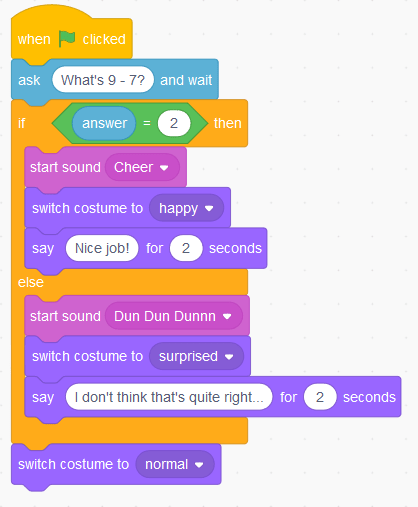
\includegraphics[width=0.9\linewidth, height=6cm]{Scratch}
\caption{scratch example}
\end{subfigure}
\begin{subfigure}{0.5\textwidth}
\rotatebox{90}{
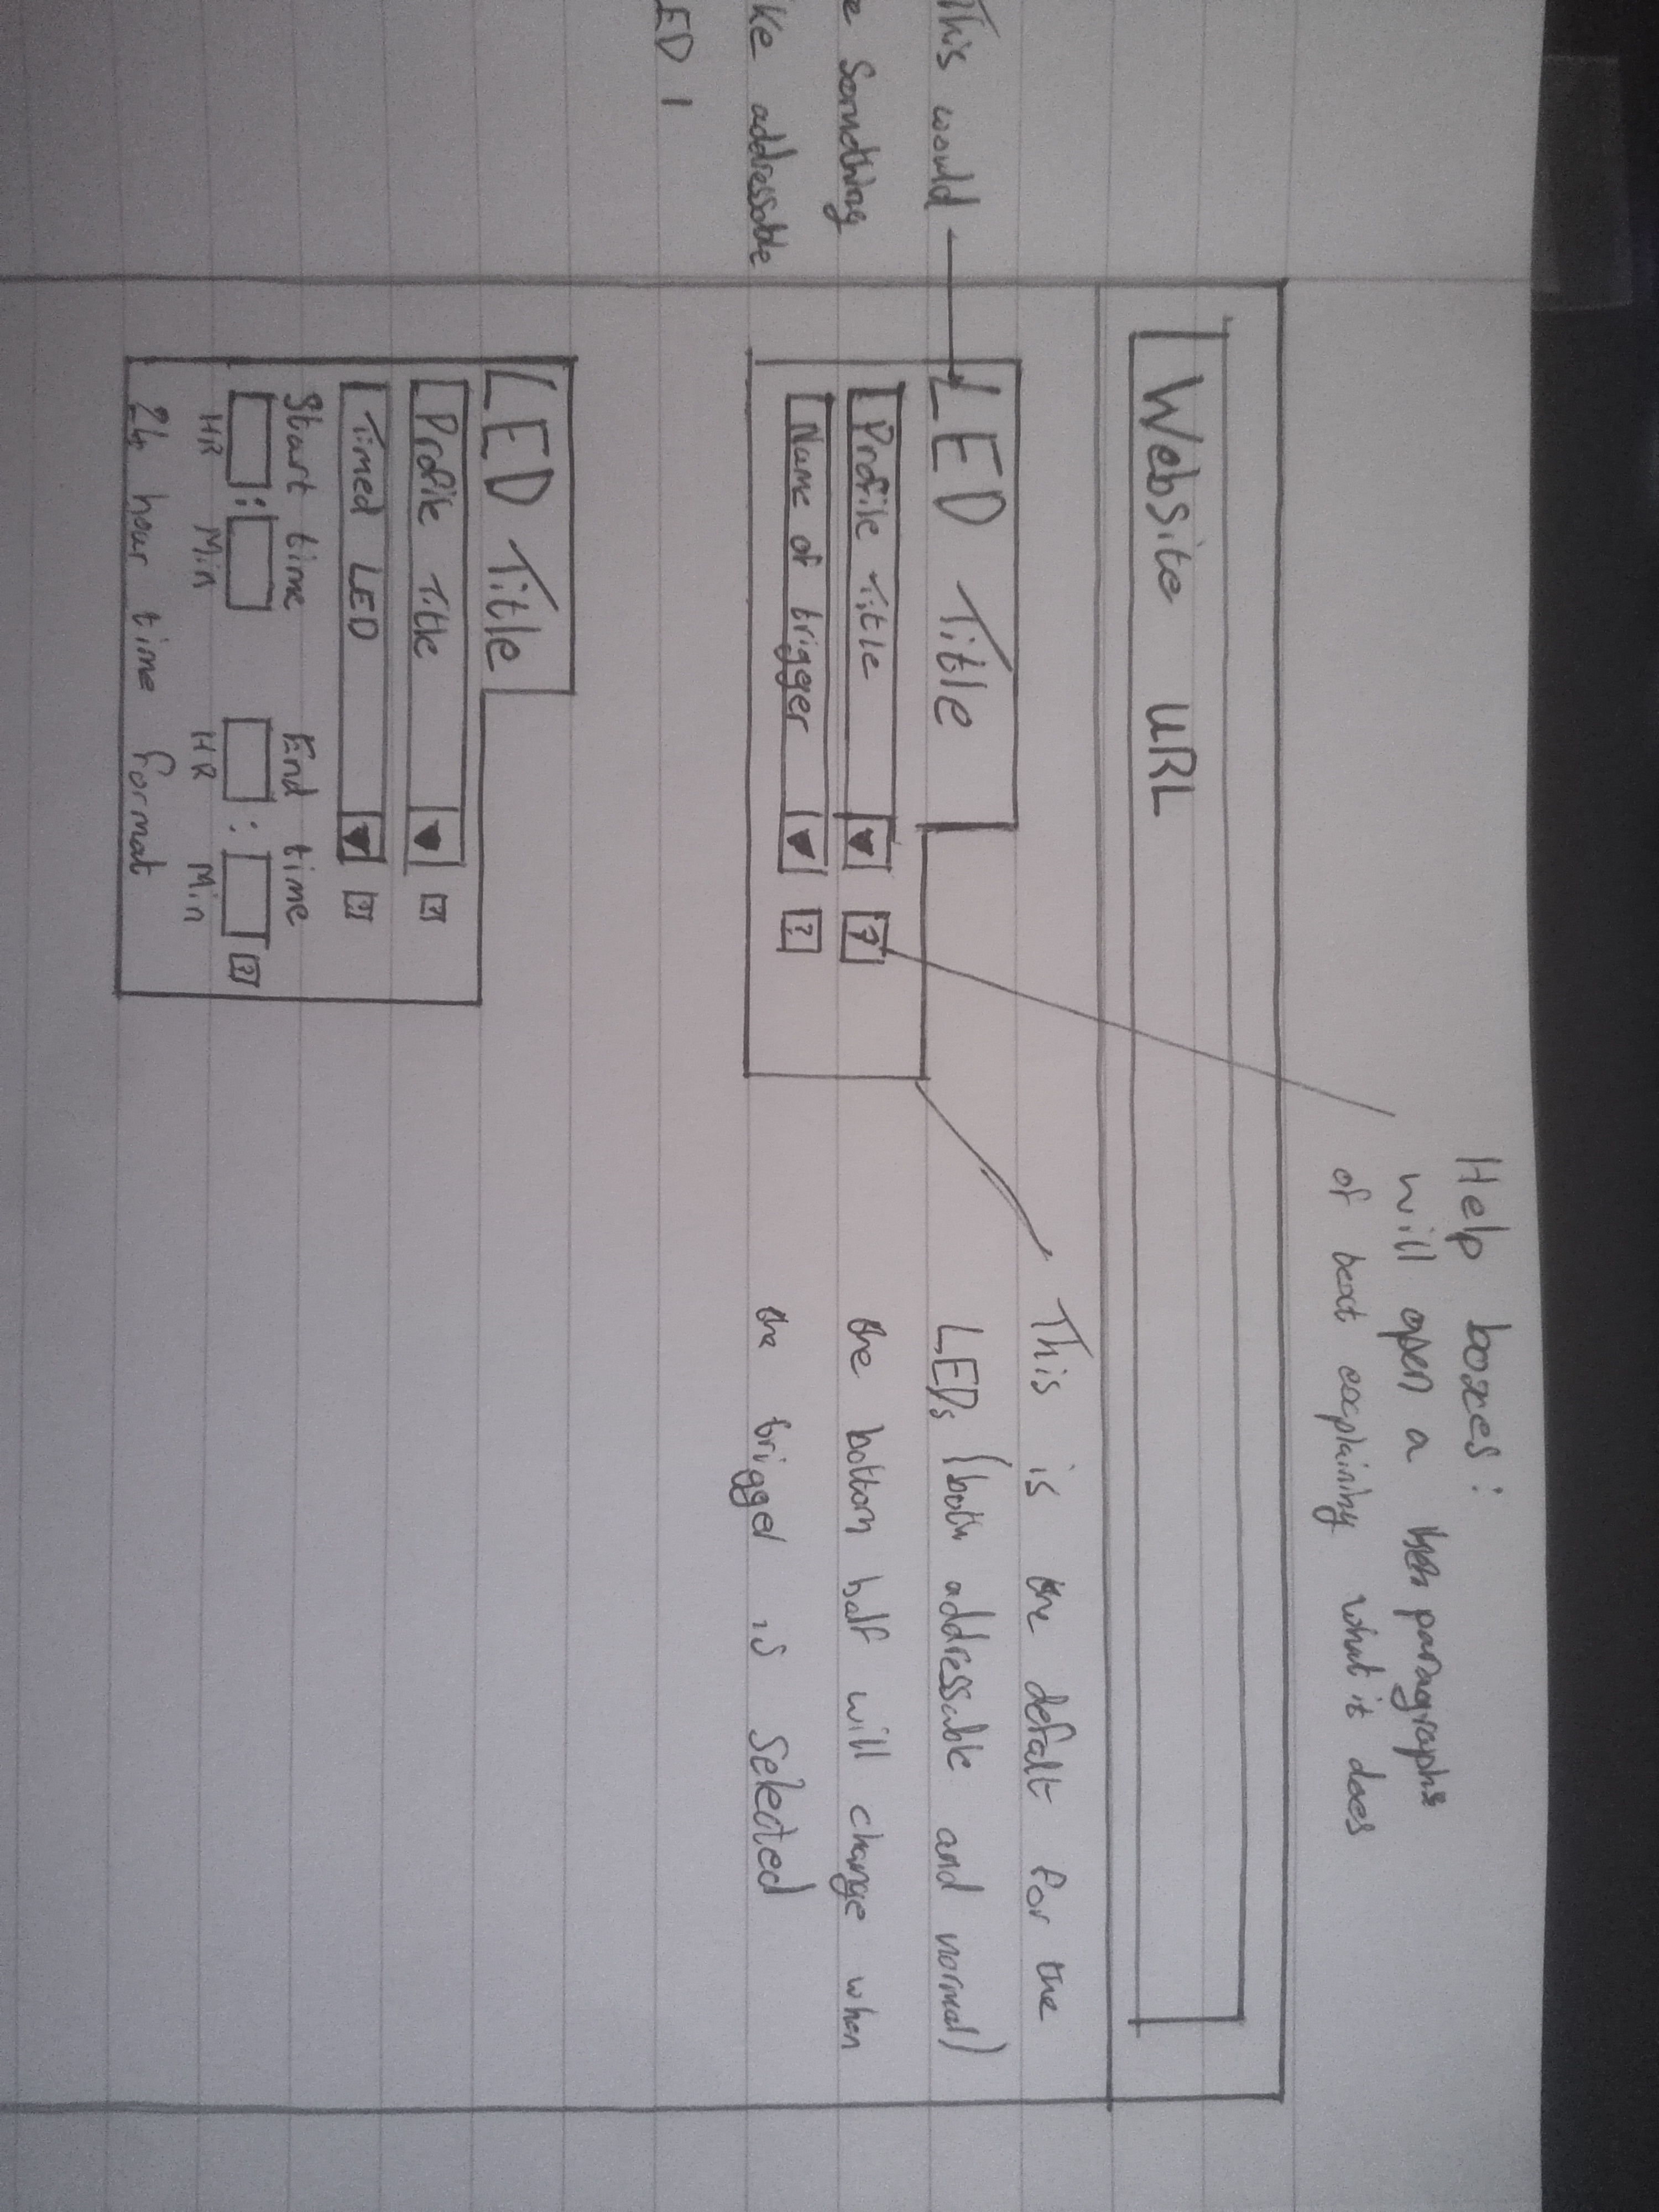
\includegraphics[width=0.8\linewidth, height=7cm]{UIDesign}}
\caption{Drawing of intended UI Design}
\end{subfigure}

\caption{Comparison Between Scratch and My UI Design}
\end{figure}

It was decided the use of code blocks, which is a similar concept on which Scratch is based on \cite{Scratch}, would make it easier for the user to understand what they were currently working on. When a trigger was chosen for the LED, additional input options were added to choose the parameters of the trigger. The additional input options depended on what trigger was chosen. For instance, if the time trigger were selected, four additional boxes appeared so that the user could enter the start and end time in hours and minutes. However, if the temperature trigger was selected, only one box would appear along with an additional drop-down box. This enabled the user to enter the threshold in which the temperature would trigger and then whether they wanted it triggering above or below this threshold. Also, to make it easier for the user to understand the expected input, there was a help box that the user could access for a description and a explanation.  This showed the user a paragraph of text explaining what they were choosing and what the expected input would look like.

\chapter{Software Design, Implementation and Testing}

This could be one chapter or a few chapters. It should define and discuss the software that is developed to support the research that is being conducted. For example, if your research involves running experiments, what software are you creating to support that work? What functionality is required? What design will be used? What implementation issues are there and what testing is used? 

Even though a research project is investigating specific research questions, it is still necessary for you to discuss the software that you develop. Research has a habit of generating bits of software that can exist for several years and need future modification. Therefore you need to be able to discuss the technical issues as well as the research approach. 

\section{Design}
You should concentrate on the more important aspects of the design. It is essential that an overview is presented before going into detail. As well as describing the design adopted it must also explain what other designs were considered and why they were rejected.

The design should describe what you expected to do, and might also explain areas that you had to revise after some investigation.

Typically, for an object-oriented design, the discussion will focus on the choice of objects and classes and the allocation of methods to classes. The use made of reusable components should be described and their source referenced. Particularly important decisions concerning data structures usually affect the architecture of a system and so should be described here.

How much material you include on detailed design and implementation will depend very much on the nature of the project. It should not be padded out. Think about the significant aspects of your system. For example, describe the design of the user interface if it is a critical aspect of your system, or provide detail about methods and data structures that are not trivial. Do not spend time on long lists of trivial items and repetitive descriptions. If in doubt about what is appropriate, speak to your supervisor.
 
You should also identify any support tools that you used. You should discuss your choice of implementation tools - programming language, compilers, database management system, program development environment, etc.

Some example sub-sections may be as follows, but the specific sections are for you to define. 

\subsection{Overall Architecture}

\subsection{Some detailed design}

\subsubsection{Even more detail}

\subsection{User Interface}

\subsection{Other relevant sections}

\section{Implementation}

This section should discuss issues you encountered as you tried to implement your experiments. What were the results of running the experiments? What conclusions can you draw from these results? 

During the work, you might have found that elements of your experiments were unnecessary or overly complex; perhaps third-party libraries were available that simplified some of the functions that you intended to implement. If things were easier in some areas, then how did you adapt your project to take account of your findings?

It is more likely that things were more complex than you first thought. In particular, were there any problems or difficulties that you found during implementation that you had to address? Did such problems simply delay you or were they more significant? 

If you had multiple experiments to run, it may be sensible to discuss each experiment in separate sections. 

\section{Testing}
Detailed descriptions of every test case are definitely not what is required in this section; the place for detailed lists of tests cases is in an appendix. In this section, it is more important to show that you adopted a sensible strategy that was, in principle, capable of testing the system adequately even if you did not have the time to test the system fully. 

Provide information in the body of your report and the appendix to explain the testing that has been performed. How does this testing address the requirements and design for the project?

How comprehensive is the testing within the constraints of the project?  Are you testing the normal working behaviour? Are you testing the exceptional behaviour, e.g. error conditions? Are you testing security issues if they are relevant for your project?

Have you tested your system on ``real users''? For example, if your system is supposed to solve a problem for a business, then it would be appropriate to present your approach to involve the users in the testing process and to record the results that you obtained. Depending on the level of detail, it is likely that you would put any detailed results in an appendix. 

Whilst testing with ``real users'' can be useful, don't see it as a way to shortcut detailed testing of your own. Think about issues discussed in the lectures about until testing, integration testing, etc. User testing without sensible testing of your own is not a useful activity.

The following sections indicate some areas you might include. Other sections may be more appropriate to your project. 

\subsection{Overall Approach to Testing}

\subsection{Automated Testing}

\subsubsection{Unit Tests}

\subsubsection{User Interface Testing}

\subsubsection{Stress Testing}

\subsubsection{Other types of testing}

\subsection{Integration Testing}

\subsection{User Testing}

\chapter{Results and Conclusions}

This section should discuss issues you encountered as you tried to implement your experiments. What were the results of running the experiments? What conclusions can you draw from these results? What graphs or other information have you assessed regarding your experiments? Discuss those.

During the work, you might have found that elements of your experiments were unnecessary or overly complex; perhaps third-party libraries were available that simplified some of the functions that you intended to implement. If things were easier in some areas, then how did you adapt your project to take account of your findings?

It is more likely that things were more complex than you first thought. In particular, were there any problems or difficulties that you found during implementation that you had to address? Did such problems simply delay you or were they more significant?

If you had multiple experiments to run, it may be sensible to discuss each experiment in separate sections.

\chapter{Evaluation}
In this chapter of the document, I have reflected upon the initial decisions made,  design plans and the overall impact and outcome of the project. 

\section{Planning}
As I took the agile methodology approach to producing the program, most of the planning phase was spent understanding what was expected of the final product and doing some spike work and experimenting mainly with hardware that I was going to use. On reflection I feel that this phase of the project is exactly what I needed to understand the scope of the project. In comparison, because most of the hardware that was being used in the project was unfamiliar to me and I have not worked with most of it before, doing a traditional waterfall style planning and design phase would not have been as helpful. This was due to a lack of experience on my part with working some of the aspects of the project. So, when it came to the implementation of the project , I would have known what I wanted the outcome to be, however I would have struggled on implementing the features desired to meet the plans specified in the design brief. This would have led to either a design brief that was not detailed enough or an over enthusiastic design document with requirements that could not have been met.

\section {Hardware Used}
Overall, I have been really impressed with the functionality of the ESP32 and the corresponding hardware (temperature sensor, regular sensor, LEDs and Ring Lights). This is due to the simplicity of how they are used and that ninety percent of the time I did not have any problems with them. From past projects, where I have used other microcontrollers and hardware, most of the time numerous hours were wasted getting the hardware to connect properly and for the code to start reading in the values before you can actually start coding with it. With every piece of hardware used on this project, the setup took at most thirty minutes before I could actually start sending/retrieving data to the different types of hardware used. I am usure whether this simplicity came from the libraries I used for the different pieces of hardware, the guides I was using [link to guides] or was lucky with good hardware but overall I am very happy with how the hardware operated with my code.

\section {Requirements}
In the planning stage of the project, the MoSCoW analysis that was recommended by my supervisor was very helpful. It helped me identify exactly what was required for the completion of the project, what extra functionalities I could add beyond that to make the project better and what functionalities were unrealistic. 

In terms of actually meeting these requirements, I am happy that most of the ‘must have’ requirements have been met and accomplished.  I am content that  I have managed to complete some of the ‘could have’ requirements. However I am disappointed that some of the requirements that I expected the website to be able to do, I have not had time to implement (explained in Following the Methodology and Time Management). Overall I have no discerning opinion on my requirements as I have been able to implement some of the requirements that were considered "extras", while some of the expected requirements were not met on the website. In hindsight I should have stopped working on the extra triggers for the profiles and started focusing on the website, I was enjoying coding with the new hardware I had acquired and as I was already working on the triggers section of the code I thought it would not be too much effort to implement the rest. 

\section {Following the Methodology and Time Management}
The Scrum methodology chosen was ideal. It fitted well with how I normally work and when it came to the planning phase of the project, it helped me understand how I was going to complete the objectives I had planned. When it came to implementing the requirements, the daily scrum and the scrum tasks helped keep me working on the first items that were implemented at the start of the project. However, as time crept on I started doing less and less daily scrums and started to slack on the repetitive tasks that kept me on track. This caused daily task to be bundled together into weekly tasks and just doing rough estimations without any proper thought. This ended-up impacting on me significantly near the end of the project as tasks that I thought would take a week took a week and a half, and so did the next task. Therefore, it did not leave me an appropriate amount of time to work on the website, so I did not meet all of the requirements.

In hindsight one of the things that caused this backlog of work near the end of the project was due to daily tasks not being extensive enough. As one of the features of Scrum is to sprint with your task for the day, when I had finished the tasks that I was working on that day’s sprint, I considered that day finished and stopped working when ideally I could have started working on the next day’s tasks to try and get ahead. 

\section {What I Would Do Differently}
If I had to start this project again or had some advice for myself at the beginning of the project. These are the following pieces of advice I would give to myself: 

\subsection{Don’t underestimate the things you do not understand}
One of the biggest mistakes I made during the planning phase was underestimating the HTML website due to doing some basic HTML a couple years previously. Do not estimate that something is going to be easier or harder depending on a limited previous experience. Two of the biggest misconceptions I had when I started this project was that the HTML would not be that complicated at all and connecting the hardware would be very hard and time consuming. Both of these misconceptions ended up being the opposite of what I thought they were going to be. 

\subsection{Just because something is repetitive and boring does not mean it is not vital}
As discussed previously, one of the biggest flaws that happened during the implementation phase of the project was not keeping up to date with my daily scrums and weekly tasks for the Scum methodology. This caused me to be behind on work when I did not realise how far behind I actually was and for me to estimate how long work would take me when I had not made any real estimates.

\subsection{Balance your time and effort equally}
Something that did not take up too much time but is still relevant as I did spend too much time on certain functions trying to perfect them when there was no need. in particular the triggers took up more time than I should have spent on them when I could have relocated that effort into something that was troubling me or that I had not yet started. 

\section{Conclusion}
The aim of the project was to create a fully customisable LED controller for the use in dioramas and model scenarios. All things considered I feel that I have acheived this this goal. This is because the user is able to create a fully functioning, flexible lighting controller.  The final LED display produced by the lighting controller has numerous output possibilities.  The user can easily set the duration of the lighting sequence, how long the colour/brightness is displayed and have mutiple LEDs all displaying at different timescales. The user also has a range of different variable triggers that they can assign to the LEDs so that the profiles will display the lighting sequences when the desired conditions are met.  However, the user is not yet able to create LED profiles via the website. 

\subsection{If I Had More Time}
If I had more time on the project, the first things I would have to implement would be a proper web front end. To do this I would spend more time on realising how to use SPIFFS for the ESP32 and host the website properly without doing it inline so then I could do the more complicated styling with CSS and HTML to make a good looking final website. 

On reflection, if I had additional time on the project to futher enhance the outcome, the biggest functionality I would have liked to implement would be the use of servos, motors and sound. The hardest aspect of this would be implementing sound to the program as it needs extra hardware for it to work (Storage and a speaker) while the servos and motors only require the servos and motors respectively to make them work. However when these functionalities would have been implemented, this would have allowed the user futher possibilities when it came to the final display of the diorama/model. 




% add any additional chapters here

%TC:ignore
\setemptyheader

%\nocite{Scrum} % include everything from the bibliography, irrespective of whether it has been referenced.

% the following line is included so that the bibliography is also shown in the table of contents. There is the possibility that this is added to the previous page for the bibliography. To address this, a newline is added so that it appears on the first page for the bibliography. 
\addcontentsline{toc}{chapter}{Annotated Bibliography} % Adds References to contents page

%
% example of including an annotated bibliography. The current style is an author date one. If you want to change, comment out the line and uncomment the subsequent line. You should also modify the packages included at the top (see the notes earlier in the file) and then trash your aux files and re-run. 
%\bibliographystyle{StylesAndReferences/authordate2annot}
\bibliographystyle{StylesAndReferences/IEEEannotU}
\renewcommand{\bibname}{Annotated Bibliography} 

\bibliography{StylesAndReferences/references} % References file


\setemptyheader

\addcontentsline{toc}{chapter}{Appendices}
\chapter*{Appendices}
\section{Original MoSCoW analysis}

Requirements 

MoSCoW – Must have (M), should have (S), could have (C) and will not have (W)

RQ1 - ESP 32 must react to the changes made by the user (M)

RQ2 - Display the brightness and the colours of the LEDs correctly (M)

RQ3 - Perform defined output when trigger is met. (M) The triggers are: 

RQ3.1 - Time 	(S)

RQ3.2 - Weather (C)

RQ3.3 - Temperature (C)

RQ3.4 - Button (C)

RQ3.5 - Sensor (C)

RQ4 - Will have 2-3 pre-set standard and addressable profiles for fire, constant and strobe(W)

RQ5 - Play MP3 file when trigger is met (W)

RQ6 - Will have some sort of storage like an SD card to store the MP3 audio (W)

RQ7 - The ESP must be easy to set up (M)



RQ8 - Create a user-friendly website.(M)

RQ9 - Easy to use and navigate (S)

RQ10 - Define the ‘trigger’ for the outputs implemented. (S)

RQ11 - Create LED standard profiles (Standard LED profiles are the brightness that must be displayed to the user e.g. PWM) (M)

RQ12 - Set the standard LED profiles to the LEDs (M)

RQ13 - Create Assignable LED profiles (Same as the standard profiles however you can set the colour of the LED) (M)

RQ14 - Set the assignable LED profiles to the assignable LEDs (needs specific assignable LEDs) (M)

RQ15 - Define the intended motor and servo config  (C)

RQ16 - Upload small MP3 file to play when defined by trigger (W)

RQ117 - Will also have a profile for the servos and motors outputs (C)


\pagebreak

% start the appendix - sets up different numbering
\fancypagestyle{plain}{%
%\fancyhf{} % clear all header and footer fields
\fancyhead[L]{Appendix\ \thechapter}
\fancyhead[R]{\leftmark}}

\appendix
\fancyhead[L]{Appendix\ \thechapter}
\fancyhead[R]{\leftmark}
\fancyhead[C]{}
\fancyfoot[C]{\thepage}
\renewcommand{\headrulewidth}{0.4pt}
\renewcommand{\chaptermark}[1]{\markboth{#1}{}}

\fancyhead[L]{Appendix\ \thechapter}
\fancyhead[R]{\leftmark}
\fancyfoot[C]{{\thepage} of \pageref{LastPage}}

% include any appendices here
\chapter{Third-Party Code and Libraries}

Adafruit NeoPixel - The adafruit neopixel libary is used tocommunicate withe the addressable LEDs. They send an RGB colour value to the LED and it displays the appropriate colour. This libary was used without modification.

WIFI - This is the libary used to host and display the website to the client. This libary was used without modification.

DHT - This is the libary used to recive values releting to the tempurture and mosture of the surrpounding environment. This libary was used without modification.
\chapter{Ethics Submission}
Ref Number
18787

AU Status
Undergraduate or PG Taught

Your aber.ac.uk email address
ktt1@aber.ac.uk

Full Name
Kieran Todd

Please enter the name of the person responsible for reviewing your assessment.
Reyer Zwiggelaar

Please enter the aber.ac.uk email address of the person responsible for reviewing
your assessment
rrz@aber.ac.uk

Supervisor or Institute Director of Research Department
cs

Module code (Only enter if you have been asked to do so)
CS39440

Proposed Study Title
ESP32 Lighting Controller

Proposed Start Date
25/01/2021

Proposed Completion Date
1/06/2021

Are you conducting a quantitative or qualitative research project?
Mixed Methods

Does your research require external ethical approval under the Health Research
Authority?
No

Does your research involve animals?
No

Does your research involve human participants?
No

Are you completing this form for your own research?
Yes

Does your research involve human participants?
No

Institute
IMPACS

Please provide a brief summary of your project (150 word max)
The ESP32 lighting project is a piece of software that easily gives the user a way of
configuring and displaying multiple different LED and motor sequences when a condition
is met for the use in models (e.g. model trains, book nooks, etc.). The lighting controller
will have an easy-to-use web-based front end for the user to assign lighting profiles to
the different LEDs and the conditions they will start lighting up under, when and how
motors will spin, and to create and edit lighting profiles that the LEDs display.

Where appropriate, do you have consent for the publication, reproduction or use of
any unpublished material?
Not applicable

\fancypagestyle{plain}{%
   \fancyhead{} %[C]{Annotated Bibliography}
   \fancyfoot[C]{{\thepage} of \pageref{LastPage}} % except the center
   \renewcommand{\headrulewidth}{0pt}
   \renewcommand{\footrulewidth}{0pt}
}

%TC:endignore

\end{document}
